\documentclass[]{article}
\usepackage{amsmath}
\usepackage{amsfonts}
\usepackage{amssymb}
\usepackage{mathtools}
\usepackage{fullpage}
\usepackage{graphicx}
\usepackage{fixltx2e}
\usepackage{listings}
\usepackage{color}
\usepackage{tikz}
\usetikzlibrary{calc,decorations.markings,shapes.misc,fadings,decorations.pathreplacing}


\tikzset{cross/.style={cross out, draw, 
         minimum size=2*(#1-\pgflinewidth), 
         inner sep=0pt, outer sep=0pt}}

\definecolor{mycolor1}{RGB}{204,51,63}
\definecolor{mycolor2}{RGB}{0,160,176}
\definecolor{mycolor3}{RGB}{217,206,178}
\long\def\/*#1*/{}
\newcommand{\HRule}{\rule{\linewidth}{0.5mm}}

\definecolor{dkgreen}{rgb}{0,0.6,0}
\definecolor{gray}{rgb}{0.5,0.5,0.5}
\definecolor{mauve}{rgb}{0.58,0,0.82}

\lstset{frame=tb,
  language=C,
  aboveskip=3mm,
  belowskip=3mm,
  showstringspaces=false,
  columns=flexible,
  basicstyle={\small\ttfamily},
  numbers=none,
  numberstyle=\tiny\color{gray},
  keywordstyle=\color{blue},
  commentstyle=\color{dkgreen},
  stringstyle=\color{mauve},
  breaklines=true,
  breakatwhitespace=true
  tabsize=3
}


\begin{document}
\begin{titlepage}
\begin{center}

\vspace*{1.0cm} 
{\huge \bfseries The properties of quantum dots formed by interstitial Mn\textsubscript{\emph{i}}\textsuperscript{2+} ions in p-i-n resonant tunneling diodes \\[0.4cm] }
\vspace{0.8cm} 

% Author and supervisor
\begin{minipage}{0.4\textwidth}
\begin{flushleft} \large
\emph{Author:}\\
Timothy \textsc{Fogarty}\textsuperscript{1}* 
\end{flushleft}
\end{minipage}
\begin{minipage}{0.4\textwidth}
\begin{flushright} \large
\emph{Supervisor:} \\
Dr.~Oleg \textsc{Makarovsky}\textsuperscript{1}
\end{flushright}
\end{minipage}
\\[0.8cm]
\textsuperscript{1}School of Physics \& Astronomy, University of Nottingham, Nottingham NG7 2RD, United Kingdom

*To whom correspondence should be addressed, pcytf@nottingham.ac.uk

\vspace{0.8cm} 
{\large \today}
\vspace{0.8cm} 

\begin{abstract}
Lorem ipsum dolor sit amet, consectetur adipiscing elit. Nulla at nisl a tellus pretium porta. Nunc dapibus mi egestas, elementum quam ut, pellentesque justo. Quisque nec purus quis lectus venenatis posuere. Vivamus bibendum neque at ante eleifend, id adipiscing felis volutpat. Proin ultrices quam nec dui consequat lacinia. Morbi lectus lectus, fringilla nec aliquet vitae, pharetra quis felis. Phasellus adipiscing faucibus bibendum. Nam aliquet felis vel lobortis accumsan. Cras ut ullamcorper lectus, ac ultricies ligula. Proin sed molestie metus, sed condimentum sem. Suspendisse in pellentesque augue. Morbi elit arcu, pharetra ac justo ac, sodales accumsan nisi. Pellentesque augue nulla, consectetur a urna porttitor, sodales malesuada purus. Fusce sit amet enim egestas, tincidunt nisl at, bibendum ante. Pellentesque dignissim ante quis auctor mollis.
\end{abstract}

\vfill

% Bottom of the page


\end{center}
\end{titlepage}

\tableofcontents

\section{Introduction}
Computers are composed of logic gates. These logic gates are the physical implementation Boolean functions $f:B^n \rightarrow B$, $B=\{0,1\}$. That is, logic gates are functions that take as input $n$ truth values and output one truth value. As such, computers are a physical implementation of a two-element Boolean algebra. Sheffer showed NAND and NOR gates are both functionally complete---that is, any logic gate could be created by a network of NAND or NOR gates. So to create a powerful computer, many NAND gates must be connected together. Doing this requires the ability to switch and amplify electrical signals. Switching means flipping bits, and is necessary to implment Boolean functions. Amplification is used to ensure electrical signals don't wane and die as they propagate through a large number of logic gates. 

The transistor is an electrical component which can both switch and amplify electrical signals. Modern computers use MOSFETs (metal-oxide-semiconductor field-effect transistors) to implement logic gates.


\section{Theory}

\subsection{Transistors}

\subsection{Doping}

\subsection{Interstitial ions}

\subsection{The potential due to a line of uniform charge}
TODO: Diagram, explain all symbols in equations, clean up text.

We search for the potential on a parallel line at a distance d from a line of uniform charge. Suppose the line of charge is composed of charges of inifinitesimal length. The potential at a single point due to the charged line is
\begin{align}
& \int \frac{1}{4\pi\epsilon_0}\frac{\text{d}q}{r}\\
= & \frac{1}{4\pi\epsilon_0} \int_{-a}^{b}\frac{\lambda \text{d}x}{\sqrt{x^2+d^2}}\\
= & \frac{\lambda}{4\pi\epsilon_0} \ln \left(\frac{b+\sqrt{b^2+d^2}}{-a+\sqrt{a^2+d^2}}\right)
\end{align}
Therefore the potential landscape defined over n points is
\begin{equation}
\sum_{i=1}^n\frac{\lambda}{4\pi\epsilon_0} \ln \left(\frac{b+\sqrt{b^2+d^2}}{-a+\sqrt{a^2+d^2}}\right)
\end{equation}
This function was implemented in MATLAB. The script was tested against a numerical model and they were found to be in agreement (see Fig).

\subsection{The potential due to a disc of uniform charge}

\subsection{Fourier transforms}

\section{Method}

\subsection{The 1D investigation}

\subsubsection{Modelling the potential landscape}


\subsubsection{The elimination of edge effects using the potential due to uniform charge}

\subsection{Optimization of code}

\subsubsection{Vectorization}

\subsubsection{Refactoring functions}
Function files provide a good way to abstract and modularize often used code. To begin with, the main computation routine of computing the potential landscapes was abstracted into a function file. However, when functions are called in matlab, the arguments are passed into the function as whole objects, not pointers. This means functions can be ineffiecient when they take a large amount of data as arguments. As all the data needs to be copied into another space in memory. This performance loss can be mitigated by using MATLAB's \texttt{lib.pointer} class, and passing a pointer into the function. However, 

\subsubsection{Parallelization}
The \texttt{for} loops in the algorithm seemed good candidates for parallelization using \texttt{parfor}. These \texttt{parfor} loops require that each iteration is independent of the others. This is the case with the potential landscape algorithm. During parallelization, MATLAB must assign iterations to the thread pool, and pass variables to each worker. This creates some overhead not present in single threaded algorithms. To make the extra overhead worth it, each iteration must be sufficiently computationally intensive. It is possible to see a linear speed-up \cite{}.

Attempting the parallelization over a pool of six workers resulted in a run time $\sim2$ times greater than the unparallelized algorithm. It is possible that each iteration, although intensive, is not intensive enough to overcome the \texttt{parfor} overhead. Hence, the single threaded algorithm was used in this model. 

\subsubsection{Refactoring loops into C with MEX files}
MATLAB is highly optimized for matrix operations. However, it is not as efficient at implementing loops as C. Given that

\lstset{language=C}  
\begin{lstlisting}
#include "mex.h"
#include <math.h>

void potential(double a, double d, double *x, double *y, double *charge, double *outMatrix, mwSize sizeX, mwSize chargeRows, mwSize sizeCharge)
{
    mwSize i,j,k;
    mwSize chargeCols = sizeCharge/chargeRows;

    for (i = 0; i < sizeX; i++) {
	for (j = 0; j < sizeX; j++) {
	    for (k = 0; k < chargeCols; k++){
		outMatrix[i + j*sizeX] += a/sqrt(pow(d, 2) + pow((x[i] - charge[k*chargeRows]), 2) + pow((y[j] - charge[1 + k*chargeRows]), 2));
	    }
	}
    }
}
\end{lstlisting}

\section{Results}

\begin{figure}
\centering
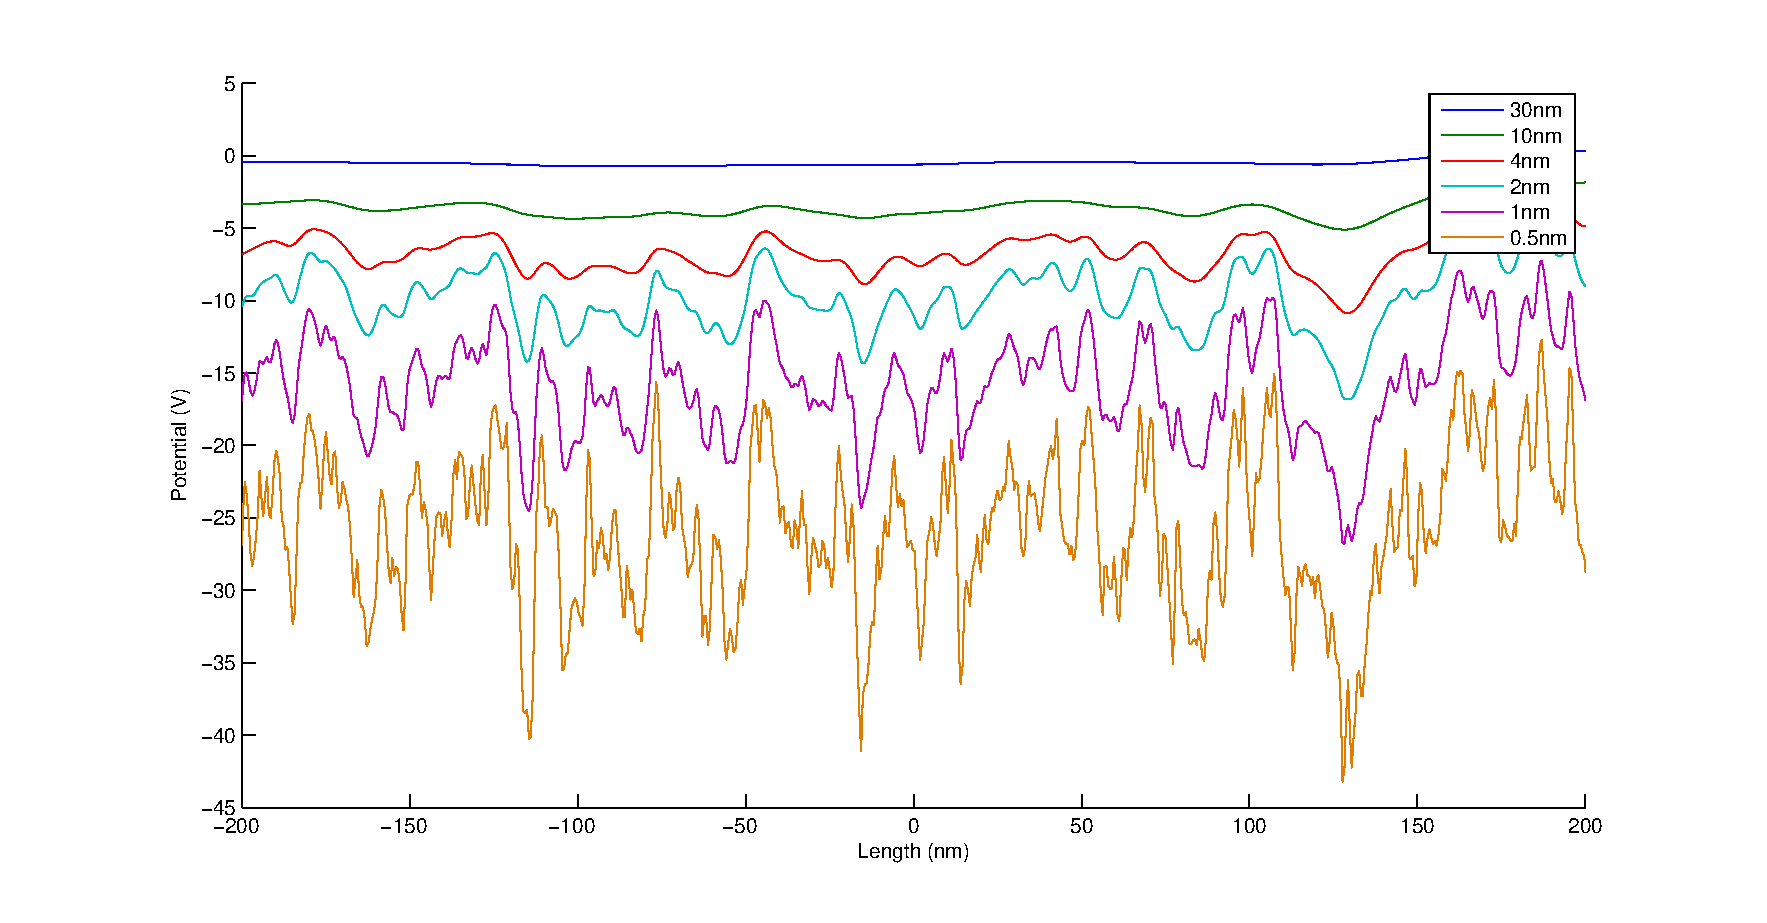
\includegraphics[width=\textwidth]{potentials.eps}
\caption{Movement of branching points in a living \emph{P. Imperitor} (a-c) at 0,1 and 2 months respectively.
Computer simulation with e being the starting and e and f being after 30,000 and 50,000 iterations \label{branching}}
\end{figure}

\begin{figure}
\centering
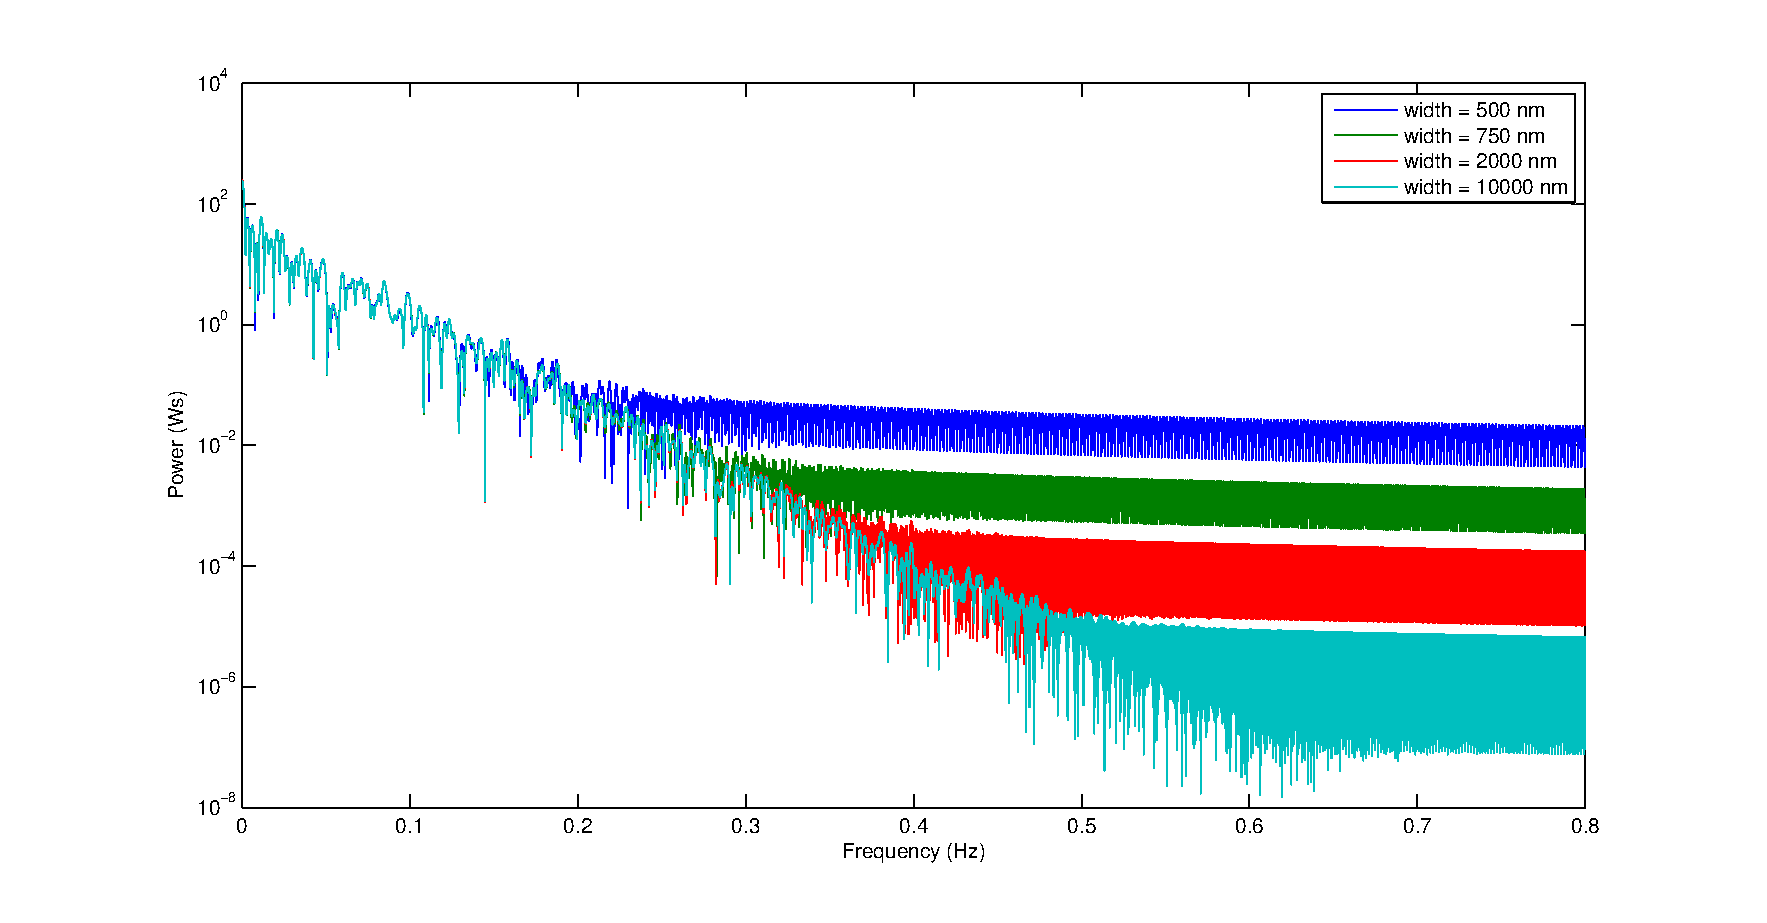
\includegraphics[width=\textwidth]{Fouriers_with_varying_range.eps}
\caption{Movement of branching points in a living \emph{P. Imperitor} (a-c) at 0,1 and 2 months respectively.
Computer simulation with e being the starting and e and f being after 30,000 and 50,000 iterations \label{branching}}
\end{figure}

\begin{figure}
\centering
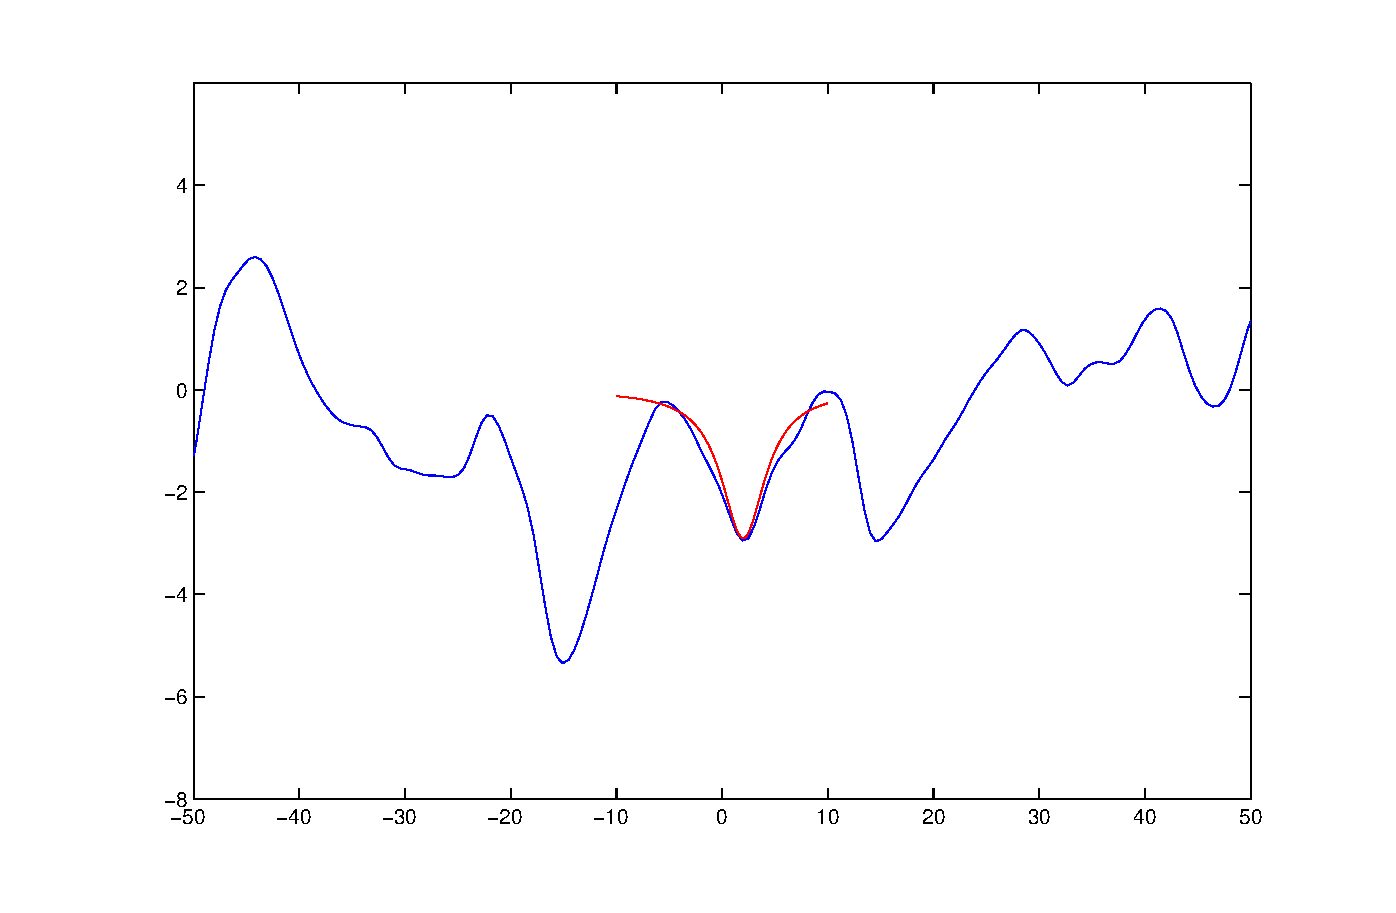
\includegraphics[width=\textwidth]{lorentzianOnLandscape.eps}
\caption{Movement of branching points in a living \emph{P. Imperitor} (a-c) at 0,1 and 2 months respectively.
Computer simulation with e being the starting and e and f being after 30,000 and 50,000 iterations \label{branching}}
\end{figure}

\begin{figure}
\centering
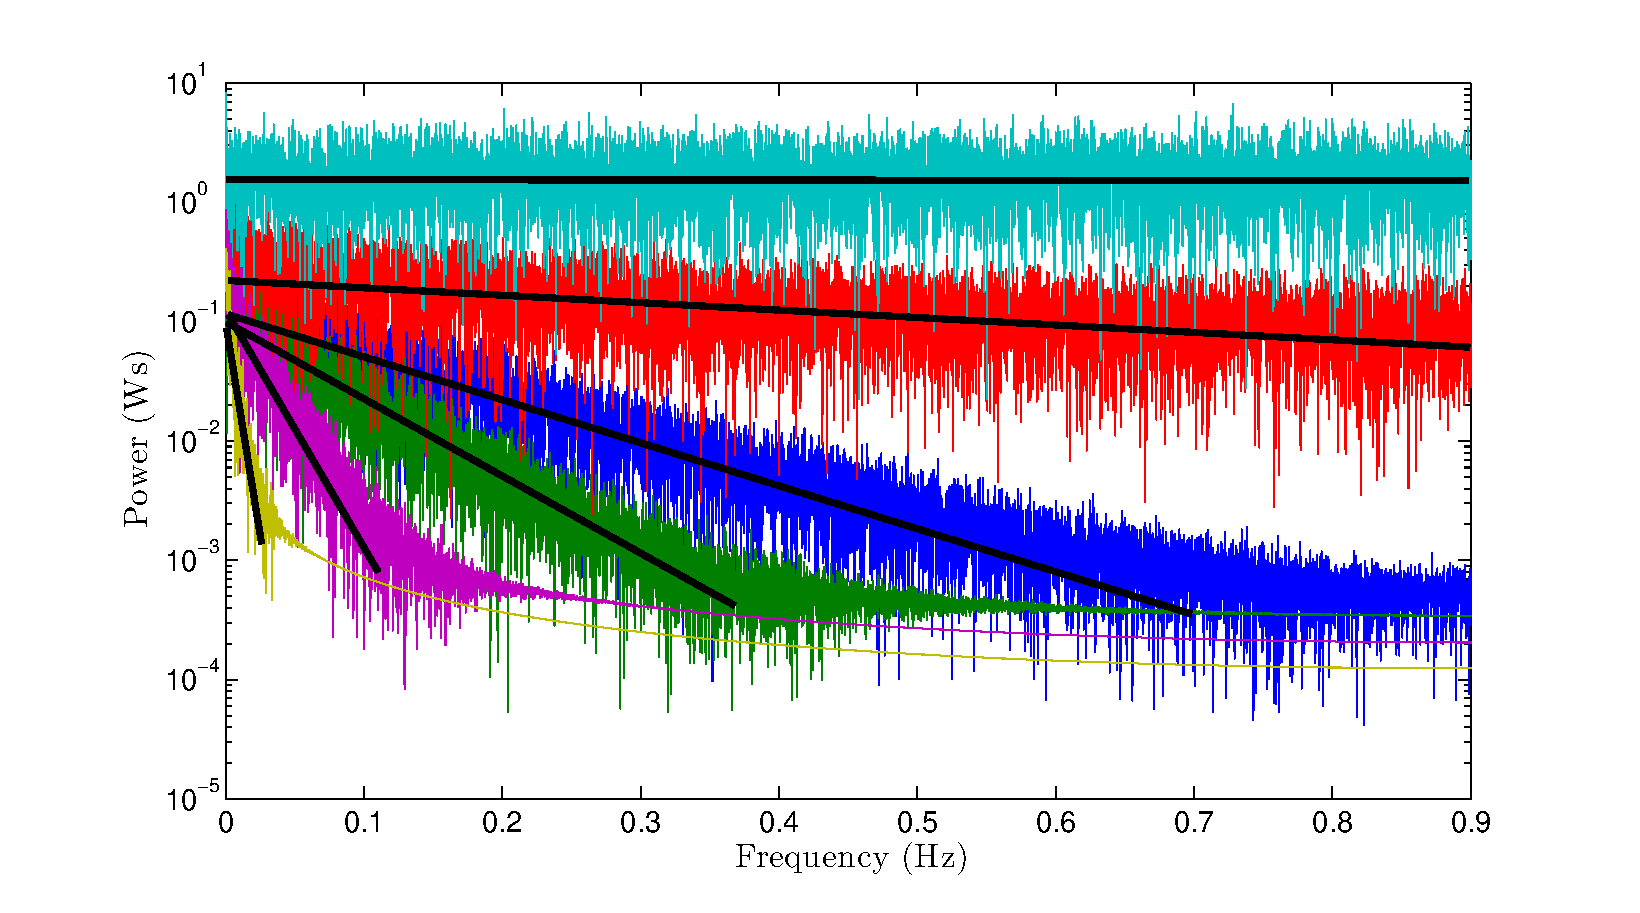
\includegraphics[width=\textwidth]{Fourier_plots_with_varying_d.eps}
\caption{Movement of branching points in a living \emph{P. Imperitor} (a-c) at 0,1 and 2 months respectively.
Computer simulation with e being the starting and e and f being after 30,000 and 50,000 iterations \label{branching}}
\end{figure}

\begin{figure}
\centering
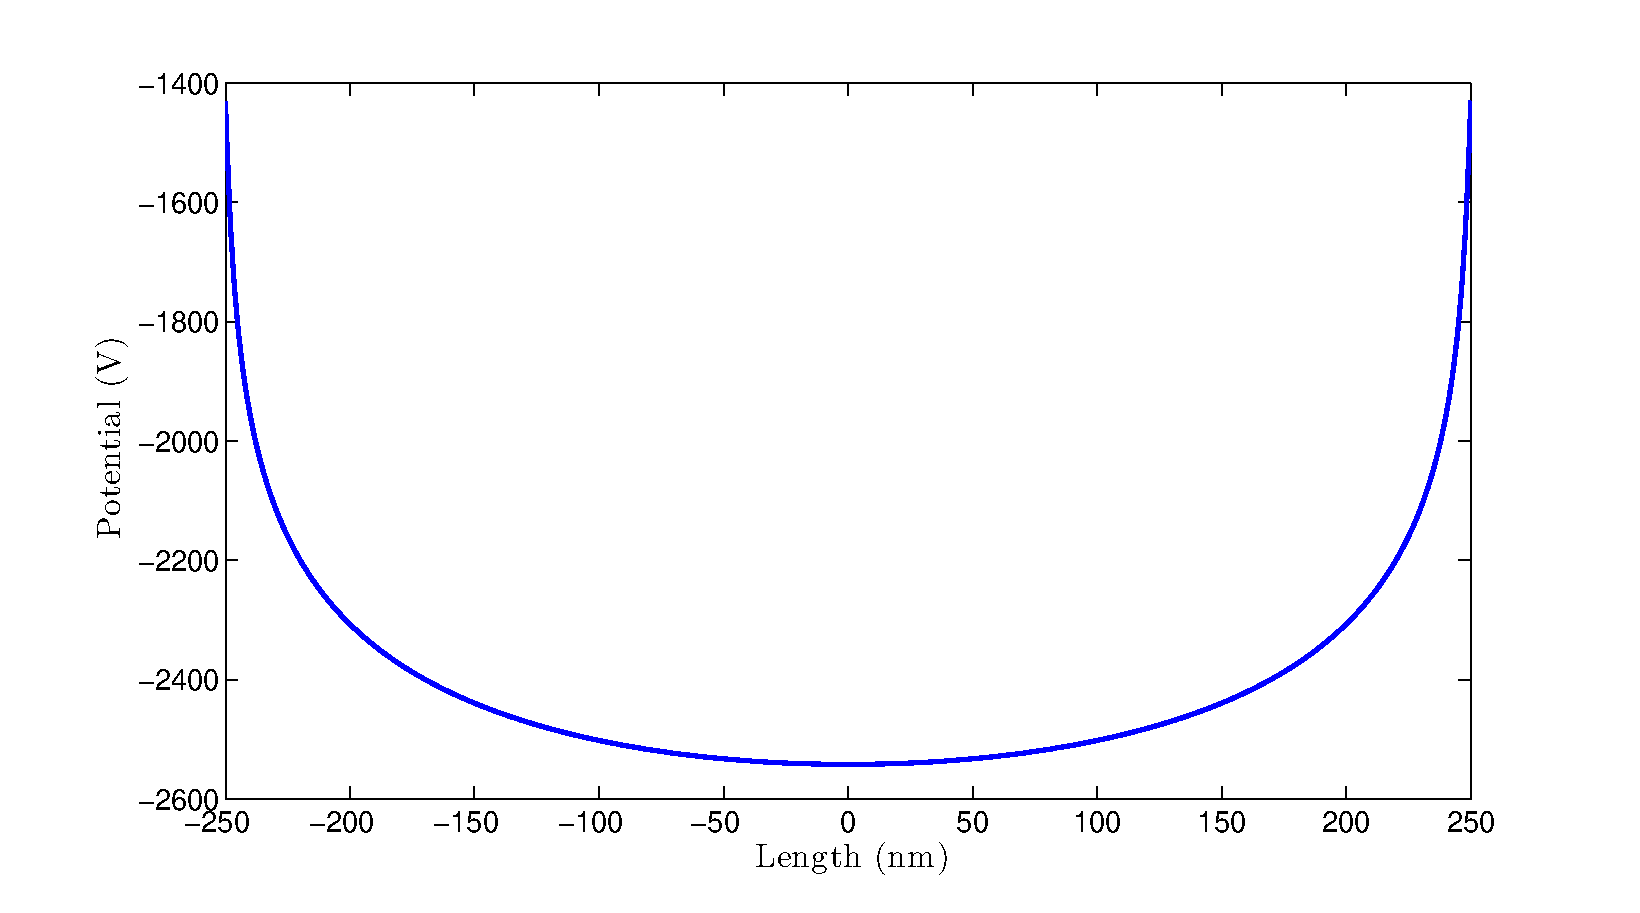
\includegraphics[width=\textwidth]{1d_Uniform_Potential.eps}
\caption{Movement of branching points in a living \emph{P. Imperitor} (a-c) at 0,1 and 2 months respectively.
Computer simulation with e being the starting and e and f being after 30,000 and 50,000 iterations \label{branching}}
\end{figure}

\begin{figure}
\centering
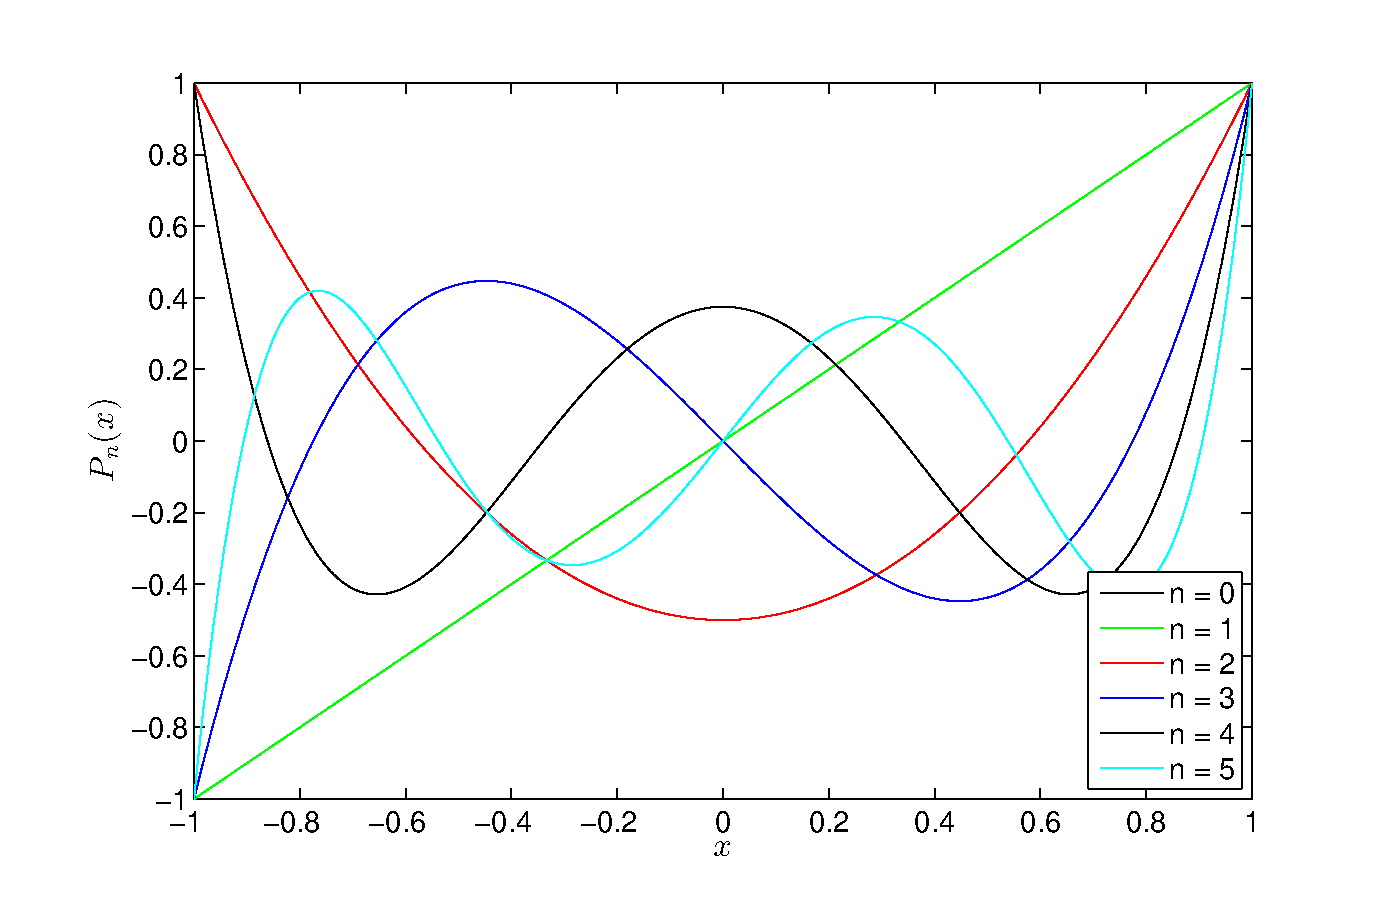
\includegraphics[width=\textwidth]{LegendrePolynomials.eps}
\caption{Movement of branching points in a living \emph{P. Imperitor} (a-c) at 0,1 and 2 months respectively.
Computer simulation with e being the starting and e and f being after 30,000 and 50,000 iterations \label{branching}}
\end{figure}

\begin{figure}
\centering
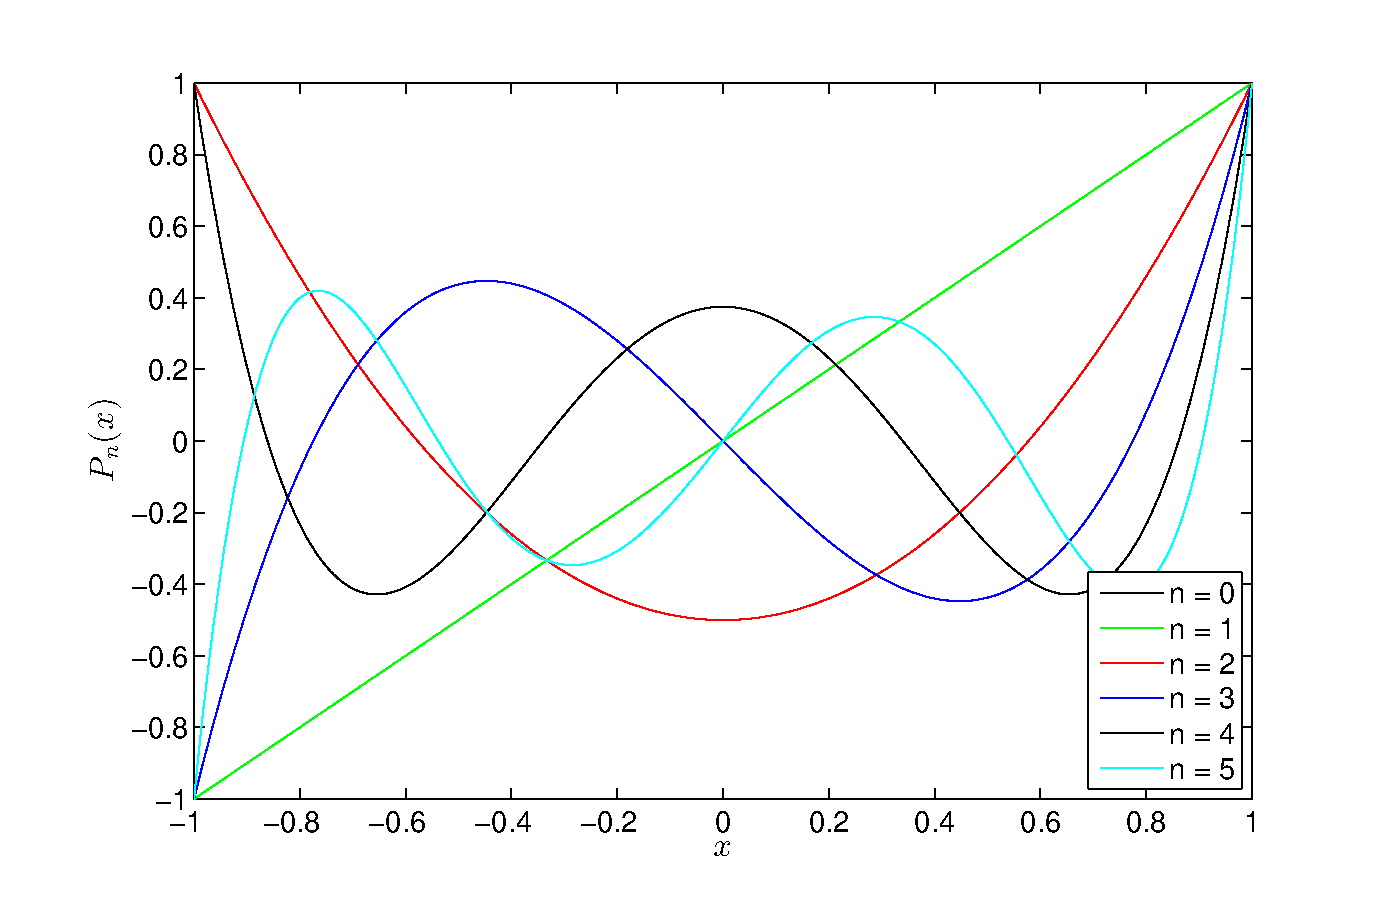
\includegraphics[width=\textwidth]{LegendrePolynomials.eps}
\caption{Movement of branching points in a living \emph{P. Imperitor} (a-c) at 0,1 and 2 months respectively.
Computer simulation with e being the starting and e and f being after 30,000 and 50,000 iterations \label{branching}}
\end{figure}

\begin{figure}
\centering
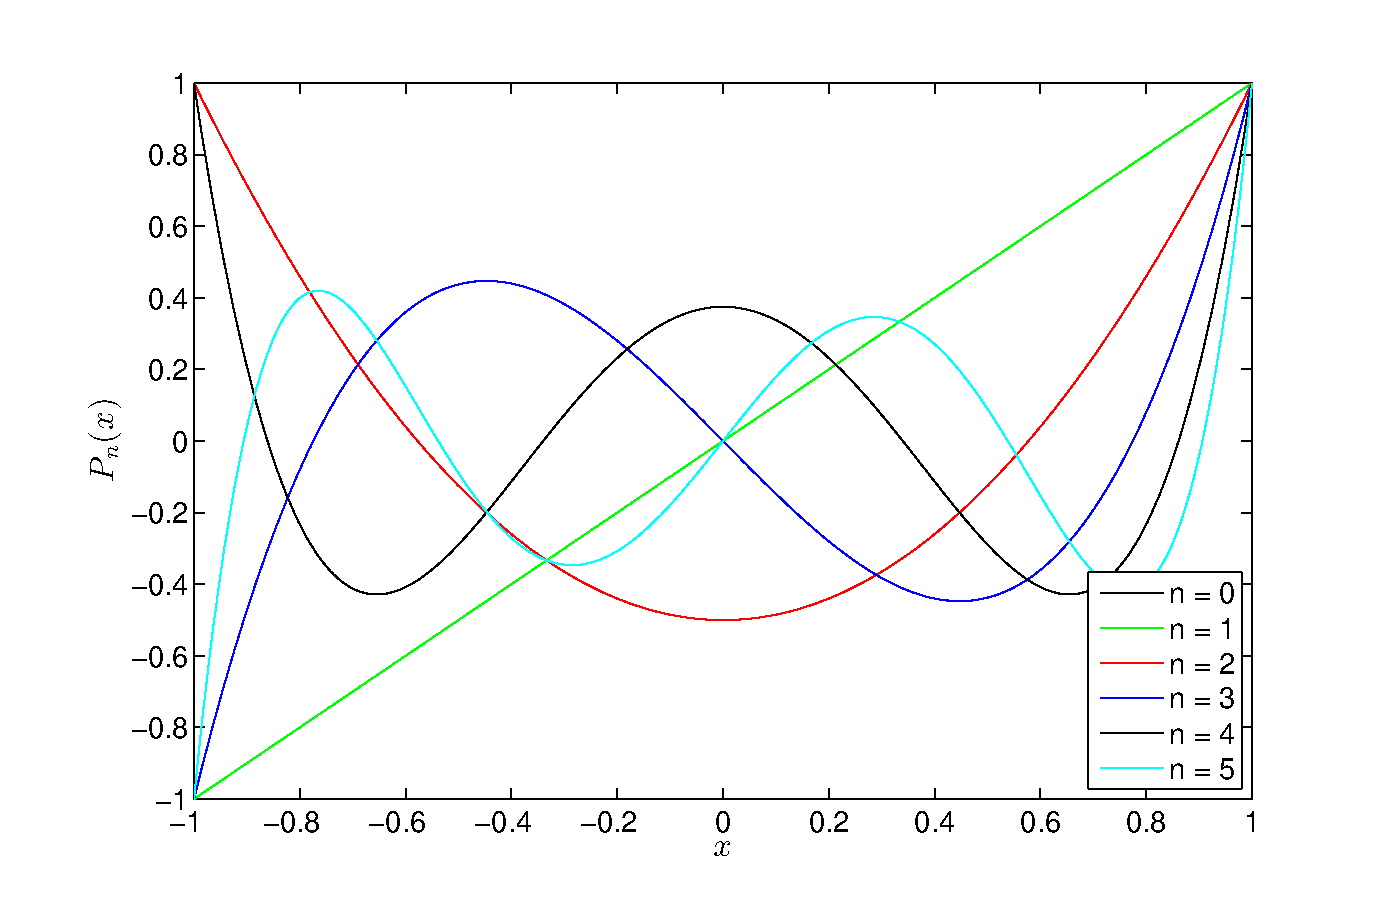
\includegraphics[width=\textwidth]{LegendrePolynomials.eps}
\caption{Movement of branching points in a living \emph{P. Imperitor} (a-c) at 0,1 and 2 months respectively.
Computer simulation with e being the starting and e and f being after 30,000 and 50,000 iterations \label{branching}}
\end{figure}

\begin{figure}
\centering
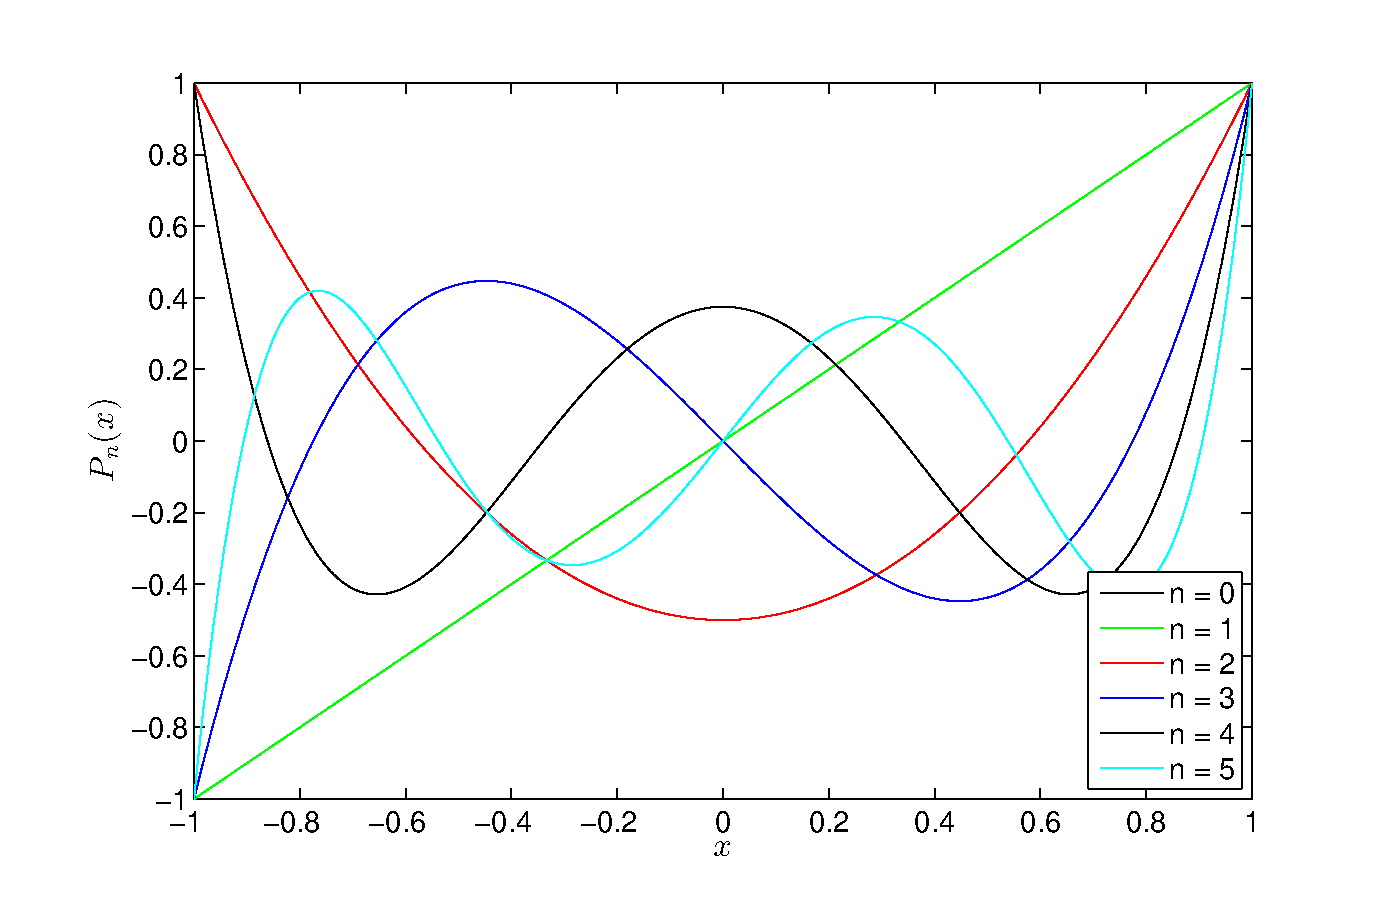
\includegraphics[width=\textwidth]{LegendrePolynomials.eps}
\caption{Movement of branching points in a living \emph{P. Imperitor} (a-c) at 0,1 and 2 months respectively.
Computer simulation with e being the starting and e and f being after 30,000 and 50,000 iterations \label{branching}}
\end{figure}

\begin{figure}
\centering
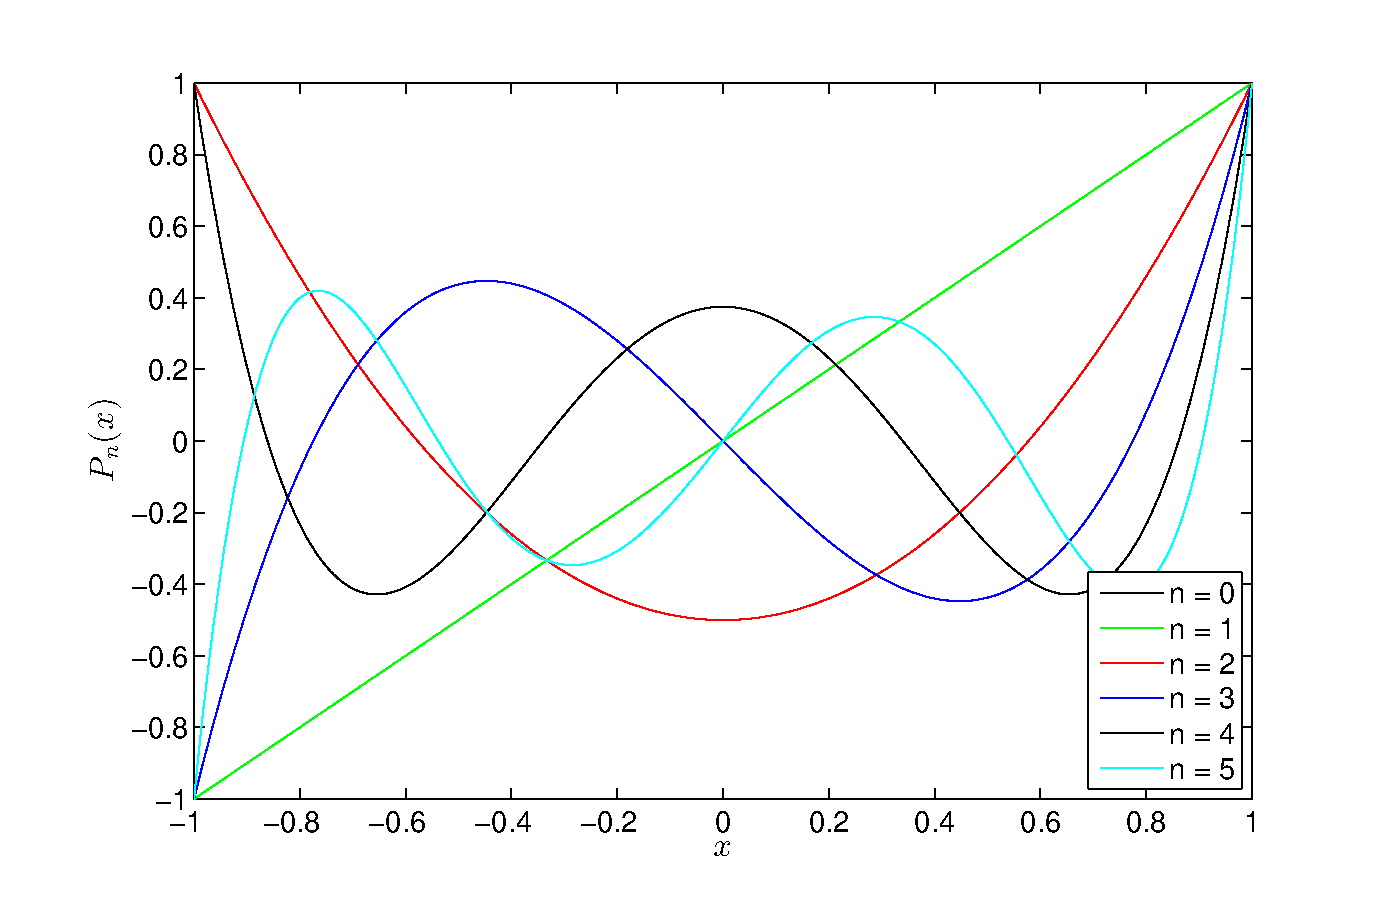
\includegraphics[width=\textwidth]{LegendrePolynomials.eps}
\caption{Movement of branching points in a living \emph{P. Imperitor} (a-c) at 0,1 and 2 months respectively.
Computer simulation with e being the starting and e and f being after 30,000 and 50,000 iterations \label{branching}}
\end{figure}


\begin{figure}
\centering
\begin{tikzpicture}
\def\nuPi{3.1459265}
\node[inner sep=0pt] (russell) at (3,-2)
    {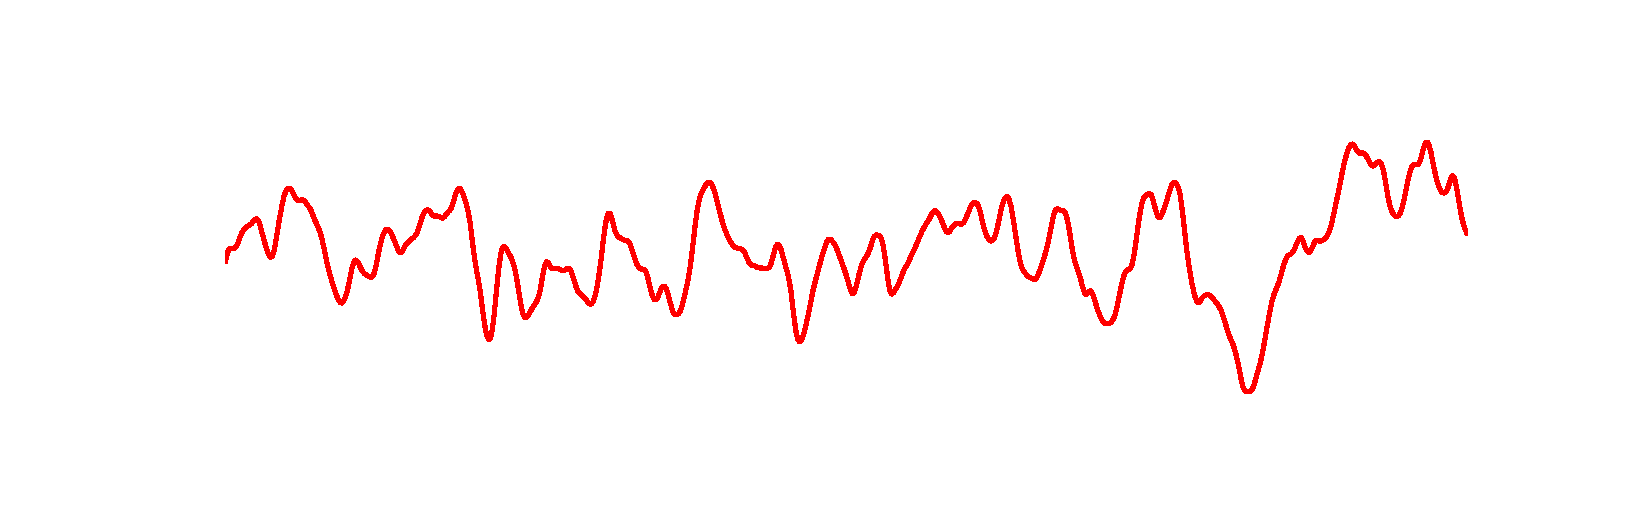
\includegraphics[width=.45\textwidth]{onelandscape.eps}};

\path [fill=mycolor1] (0,0) rectangle (6,1);
\node [white] at (3, 0.5) {p-GaAs};
\draw [thick, ->] (-0.2,0) --(-0.2,-2);
\node [left] at (-0.2,-1) {$d$};
\foreach \i in {1,2,...,30}{
  \foreach \j in {1,2,3}{
  \pgfmathsetmacro{\dx}{(rand*0.5+0.5)*6}
  \pgfmathsetmacro{\dy}{(rand*0.5+0.5)}
  \pgfmathsetmacro{\rot}{rand*0.1}   
  \shade[ball color=mycolor1] ({\dx+\rot},{-(\dy+\rot)*\j/5}) circle(0.12); 
  }
}
\draw [thick,decorate,decoration={brace,amplitude=2pt,raise=3pt},yshift=0pt]
(6.2,0) -- (6.2,-0.8) node [black,midway,xshift=0.8cm] {donors};

\path [fill=mycolor3] (0,-3) rectangle (6,-3.5);
\path [fill=mycolor3] (0,-4) rectangle (6,-4.5);

\draw [thick, <-] (5.5,-2.5) --(6.5,-3.75);
\draw [thick, <-] (5.5,-3.75) --(6.5,-3.75);
\draw [thick, <-] (5.5,-5) --(6.5,-3.75);
\node [right] at (6.5,-3.75) {i-GaAs};

\draw [thick, <-] (0.5,-3.25) --(-0.5,-3.75);
\draw [thick, <-] (0.5,-4.25) --(-0.5,-3.75);
\node [left] at (-0.5,-3.75) {AlAs};

\path [fill=mycolor2] (0,-6) rectangle (6,-7);
\node [white] at (3, -6.5) {n-GaAs};


\end{tikzpicture}
\end{figure}

\section{Discussion}

\section{Conclusion}

\section{Summary}

\bibliographystyle{unsrt}
\bibliography{mybib} 

\end{document}
